%%%%%%%%%%%%%%%%%%%%%%%%%%%%%%%%%%%%%%%%%%%%%%%%%%%%%%%%%%%%%%%

\newpage
\section{Dominik Breksa - Kolej w polsce}

%%%%%%%%%%%%%%%%%%%%%%%%%%%%%%%%%%%%%%%%%%%%%%%%%%%%%%%%%%%%%%%

\subsection{Matematyka:}
$m\in\mathbb{R}$
\[
\left\{
\begin{array}{rl}
x+y &=\:\:2m-1 \\
x^2+y^2&=\:\: m^2-4m+4
\end{array}
\right\}
\]

\begin{center}
    
     $$\Biggl(\biggl(\Bigl(\bigl(( a )\bigr)\Bigr)\biggr)\Biggr)$$
    Nie ma większych nawiasów, ale i tak są fajne.
     $$\left|1+\right|a-5||$$
    $ x\in R$

   `$ x\in\mathcal{R},   x\in\mathfrak{R},  x\in\mathbf{R},   x\in\mathbb{R}$

\end{center}

%%%%%%%%%%%%%%%%%%%%%%%%%%%%%%%%%%%%%%%%%%%%%%%%%%%%%%%%%%%%%%%

\subsection{Tabela informacji o lokomotywach:}
\begin{center}
\begin{table}[!ht]
\caption{Szczegółowe informacje o wybranch lokomotywach}
\label{tab:Tabela}
\begin{tabular}{@{}|c|c|c|c|c|@{}}
\toprule
\textit{\textbf{Nazwa}} & \textit{\textbf{Żargonowa nazwa}} & \textit{\textbf{Rodzaj}} & \textit{\textbf{Rok produkcji}} & \textit{\textbf{Ilość sztuk}} \\ \midrule
Pt47                         & "Petucha, Pyta"                              & L. Paro.              & 1948 - 1951                     & 180                                    \\ \midrule
Ol49                         & "Oelka, Oka"                                 & L. Paro.              & 1951 - 1954                     & 112                                    \\ \midrule
EP09                         & "Dziewiątka, Epoka"                          & L. Elek.        & 1986 - 1997                     & 47                                     \\ \midrule
EM10                         & "Krokodyl, Kangurek"                         & L. Elek.        & 1990 - 1991                     & {[}Brak danych{]}                    \\ \midrule
EU07                         & "Siódemka, Anglik"                           & L. Elek.        & 1965 - 1977                     & 240                                    \\ \midrule
SM42                         & "Stonka, Łajka"                              & L. Spal.          & 1963 - 1993                     & 1224                                   \\ \midrule
ST44                         & "Gagarin, Iwan"                              & L. Spal.          & 1965 - 1988                     & 1114                                   \\ \midrule
ST40                         & "Batman"                                     & L. Spal.           & 2007 - 2021                     & 48                                     \\ \bottomrule
\end{tabular}
\end{table}
\end{center}
\newpage

%%%%%%%%%%%%%%%%%%%%%%%%%%%%%%%%%%%%%%%%%%%%%%%%%%%%%%%%%%%%%%%

\subsection{Zdjęcia pojazdów szynowych:}
\begin{center}
\begin{figure}[!ht]
\begin{center}
 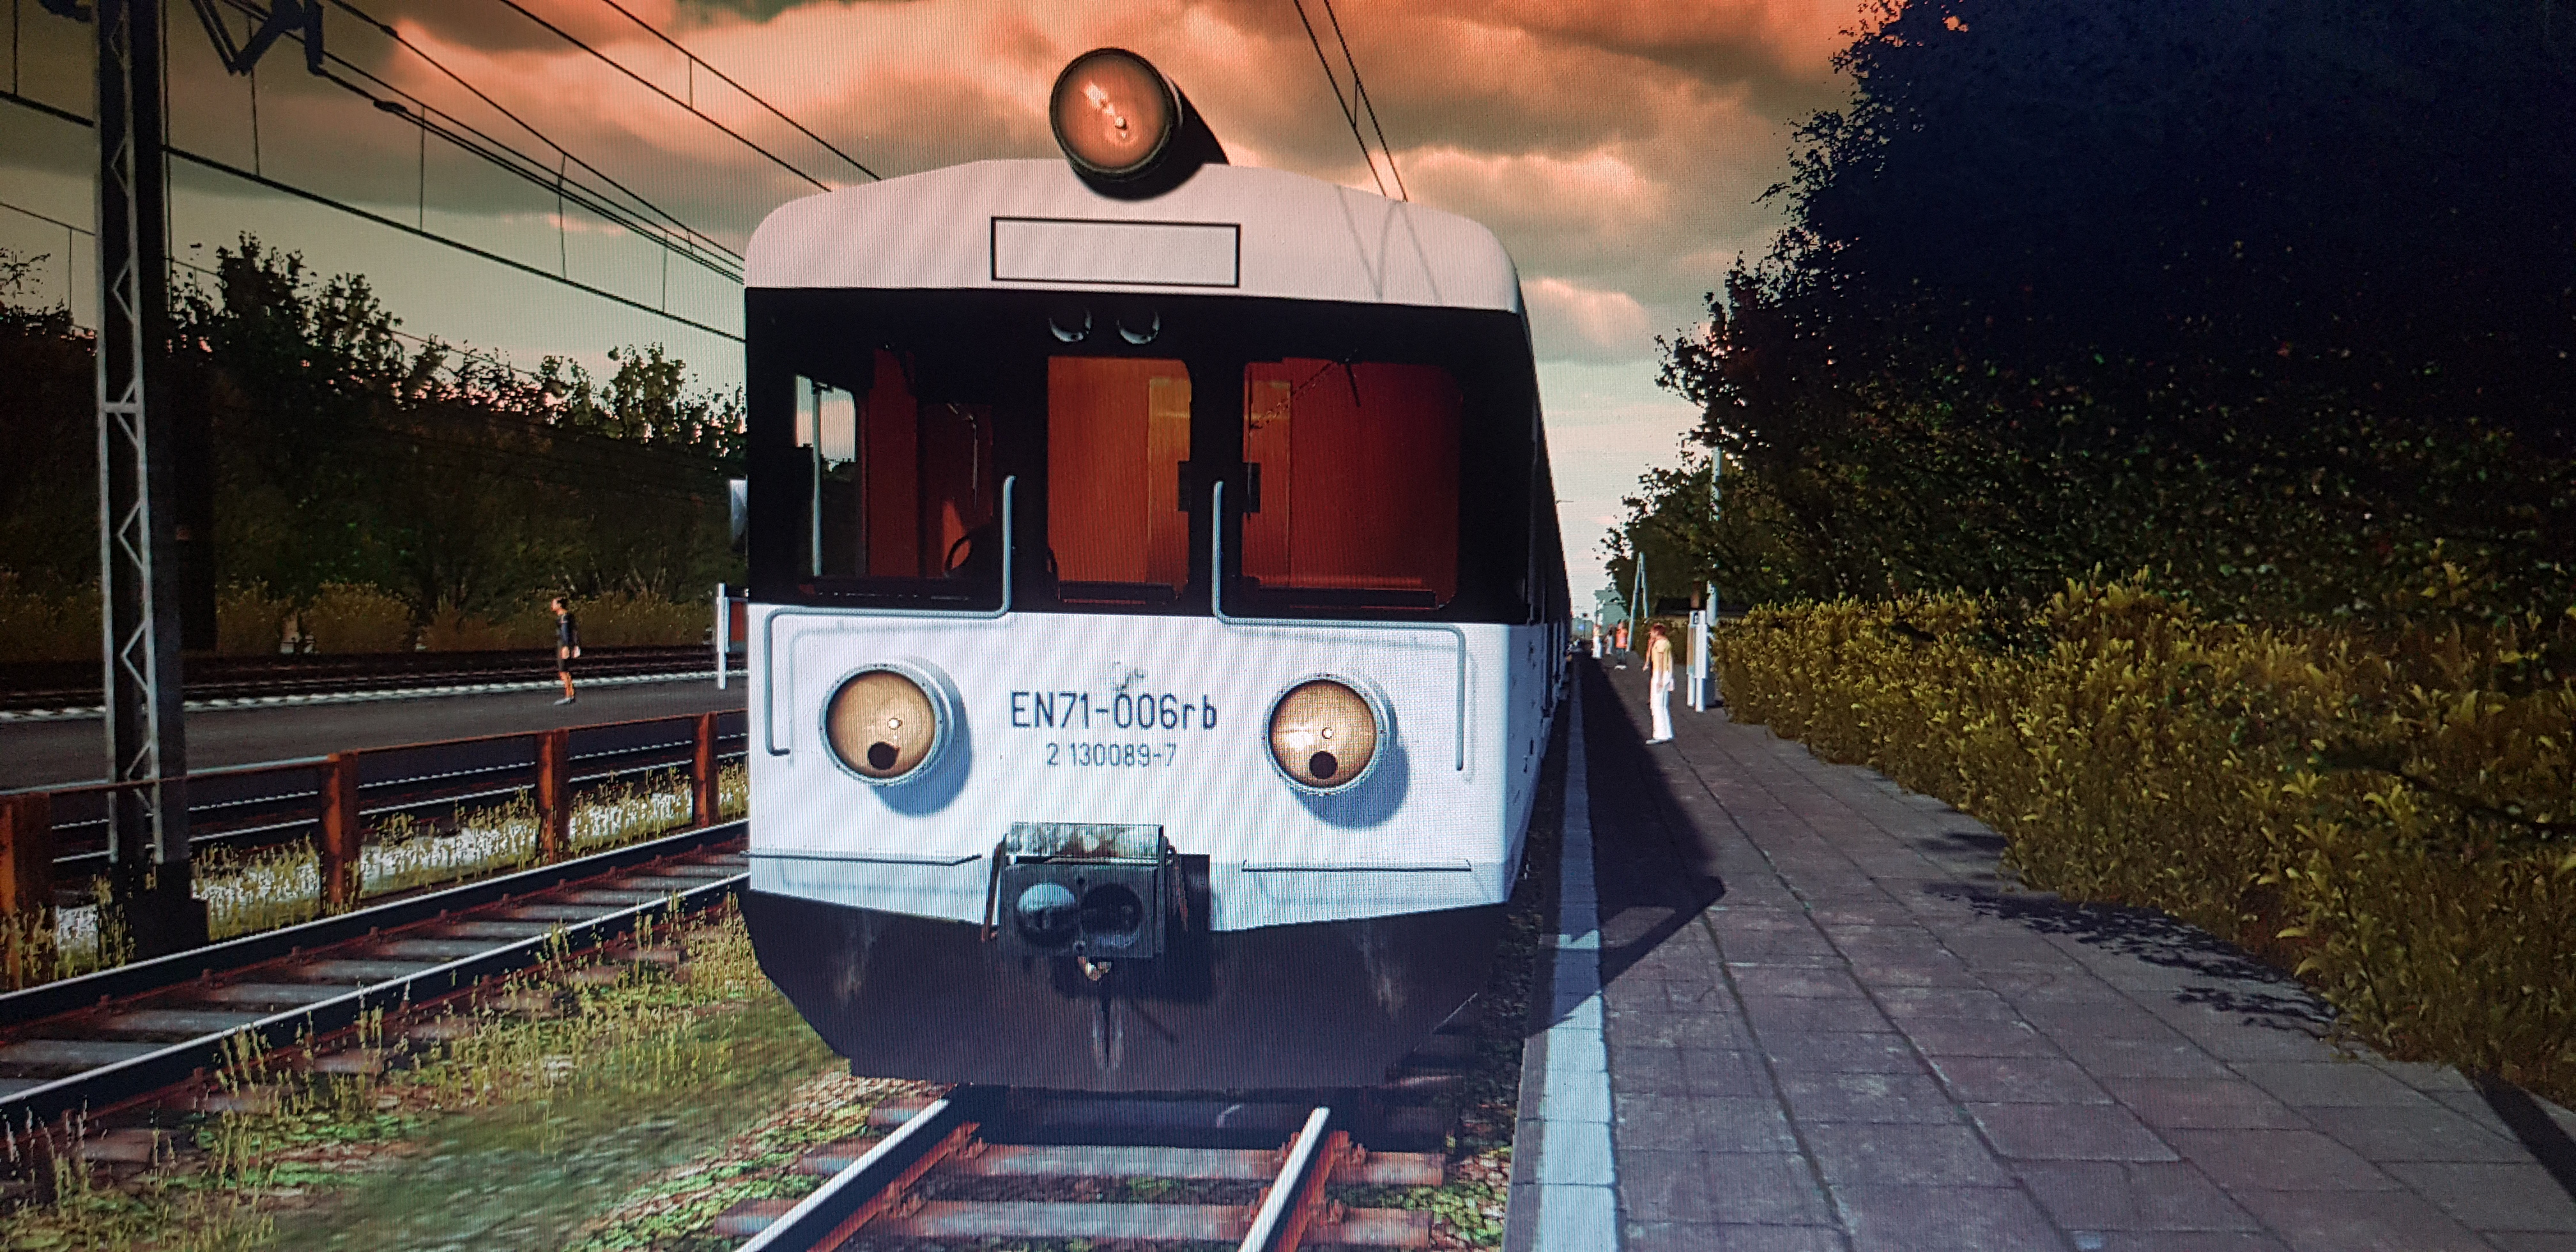
\includegraphics[width=8cm]{pictures/Dominik/20210919_185854.jpg}
  \caption{Pociąg EN71 - 006 Na szlaku}
  \label{fig:1}
\end{center}
\end{figure}
\begin{figure}[!ht]
\begin{center}
 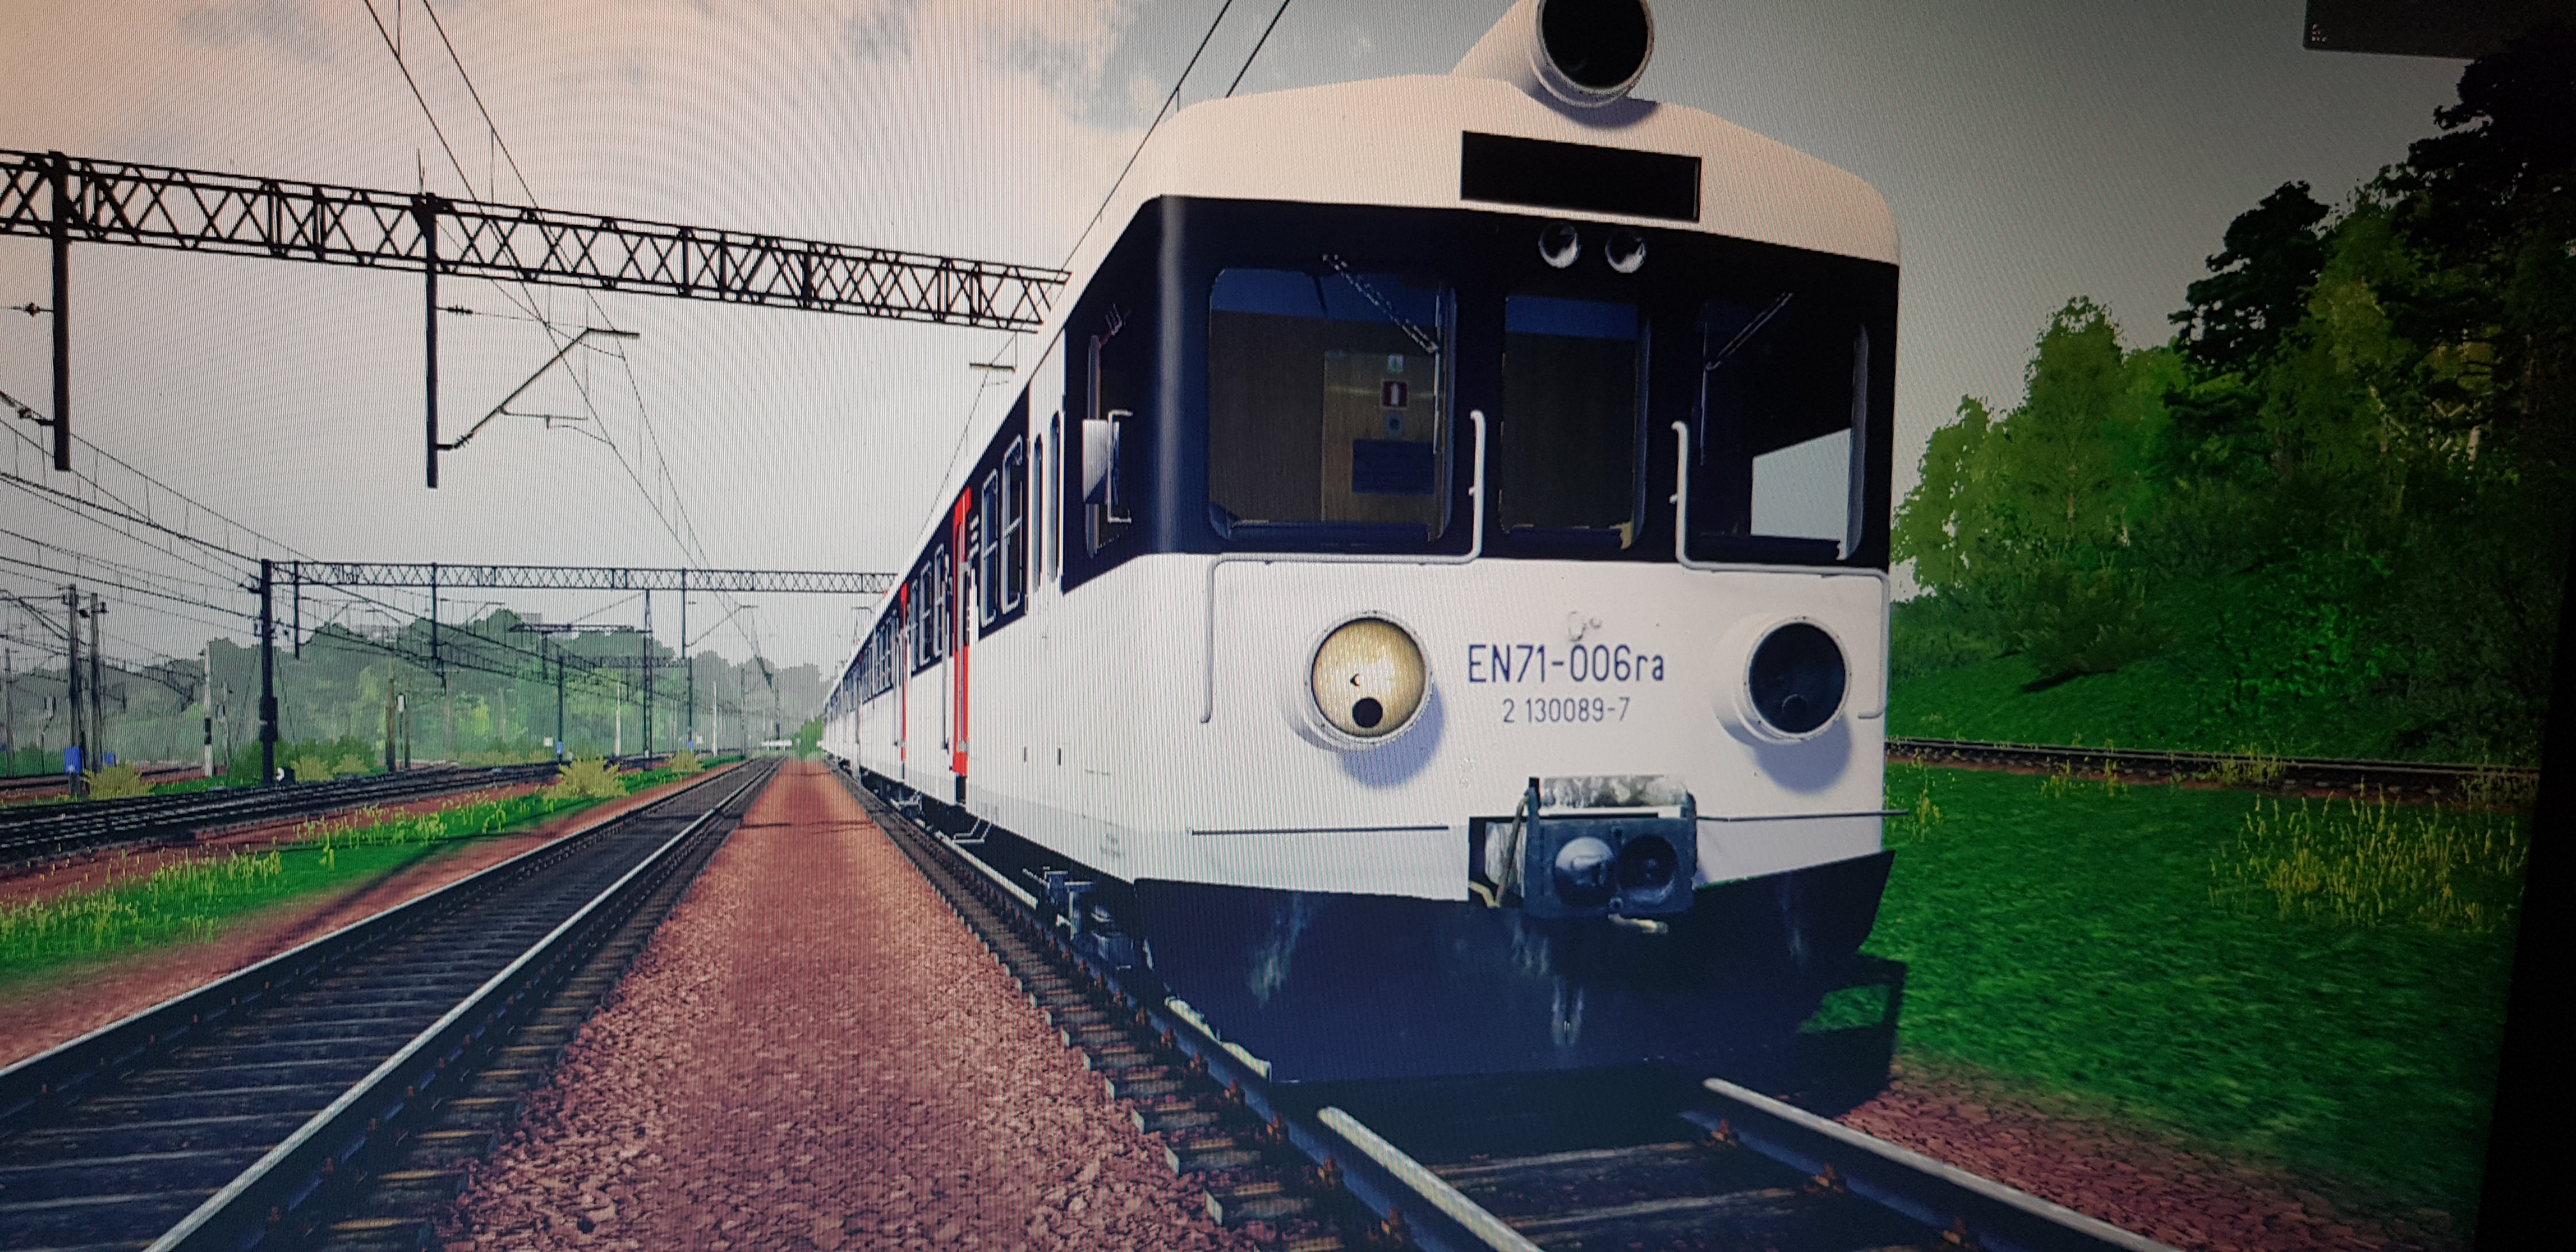
\includegraphics[width=8cm]{pictures/Dominik/20210920_224618.jpg}
  \caption{Pociąg EN71 - 006 podczas jazdy manewrowej}
  \label{fig:2}
\end{center}
\end{figure}
\begin{figure}[!ht]
\begin{center}
 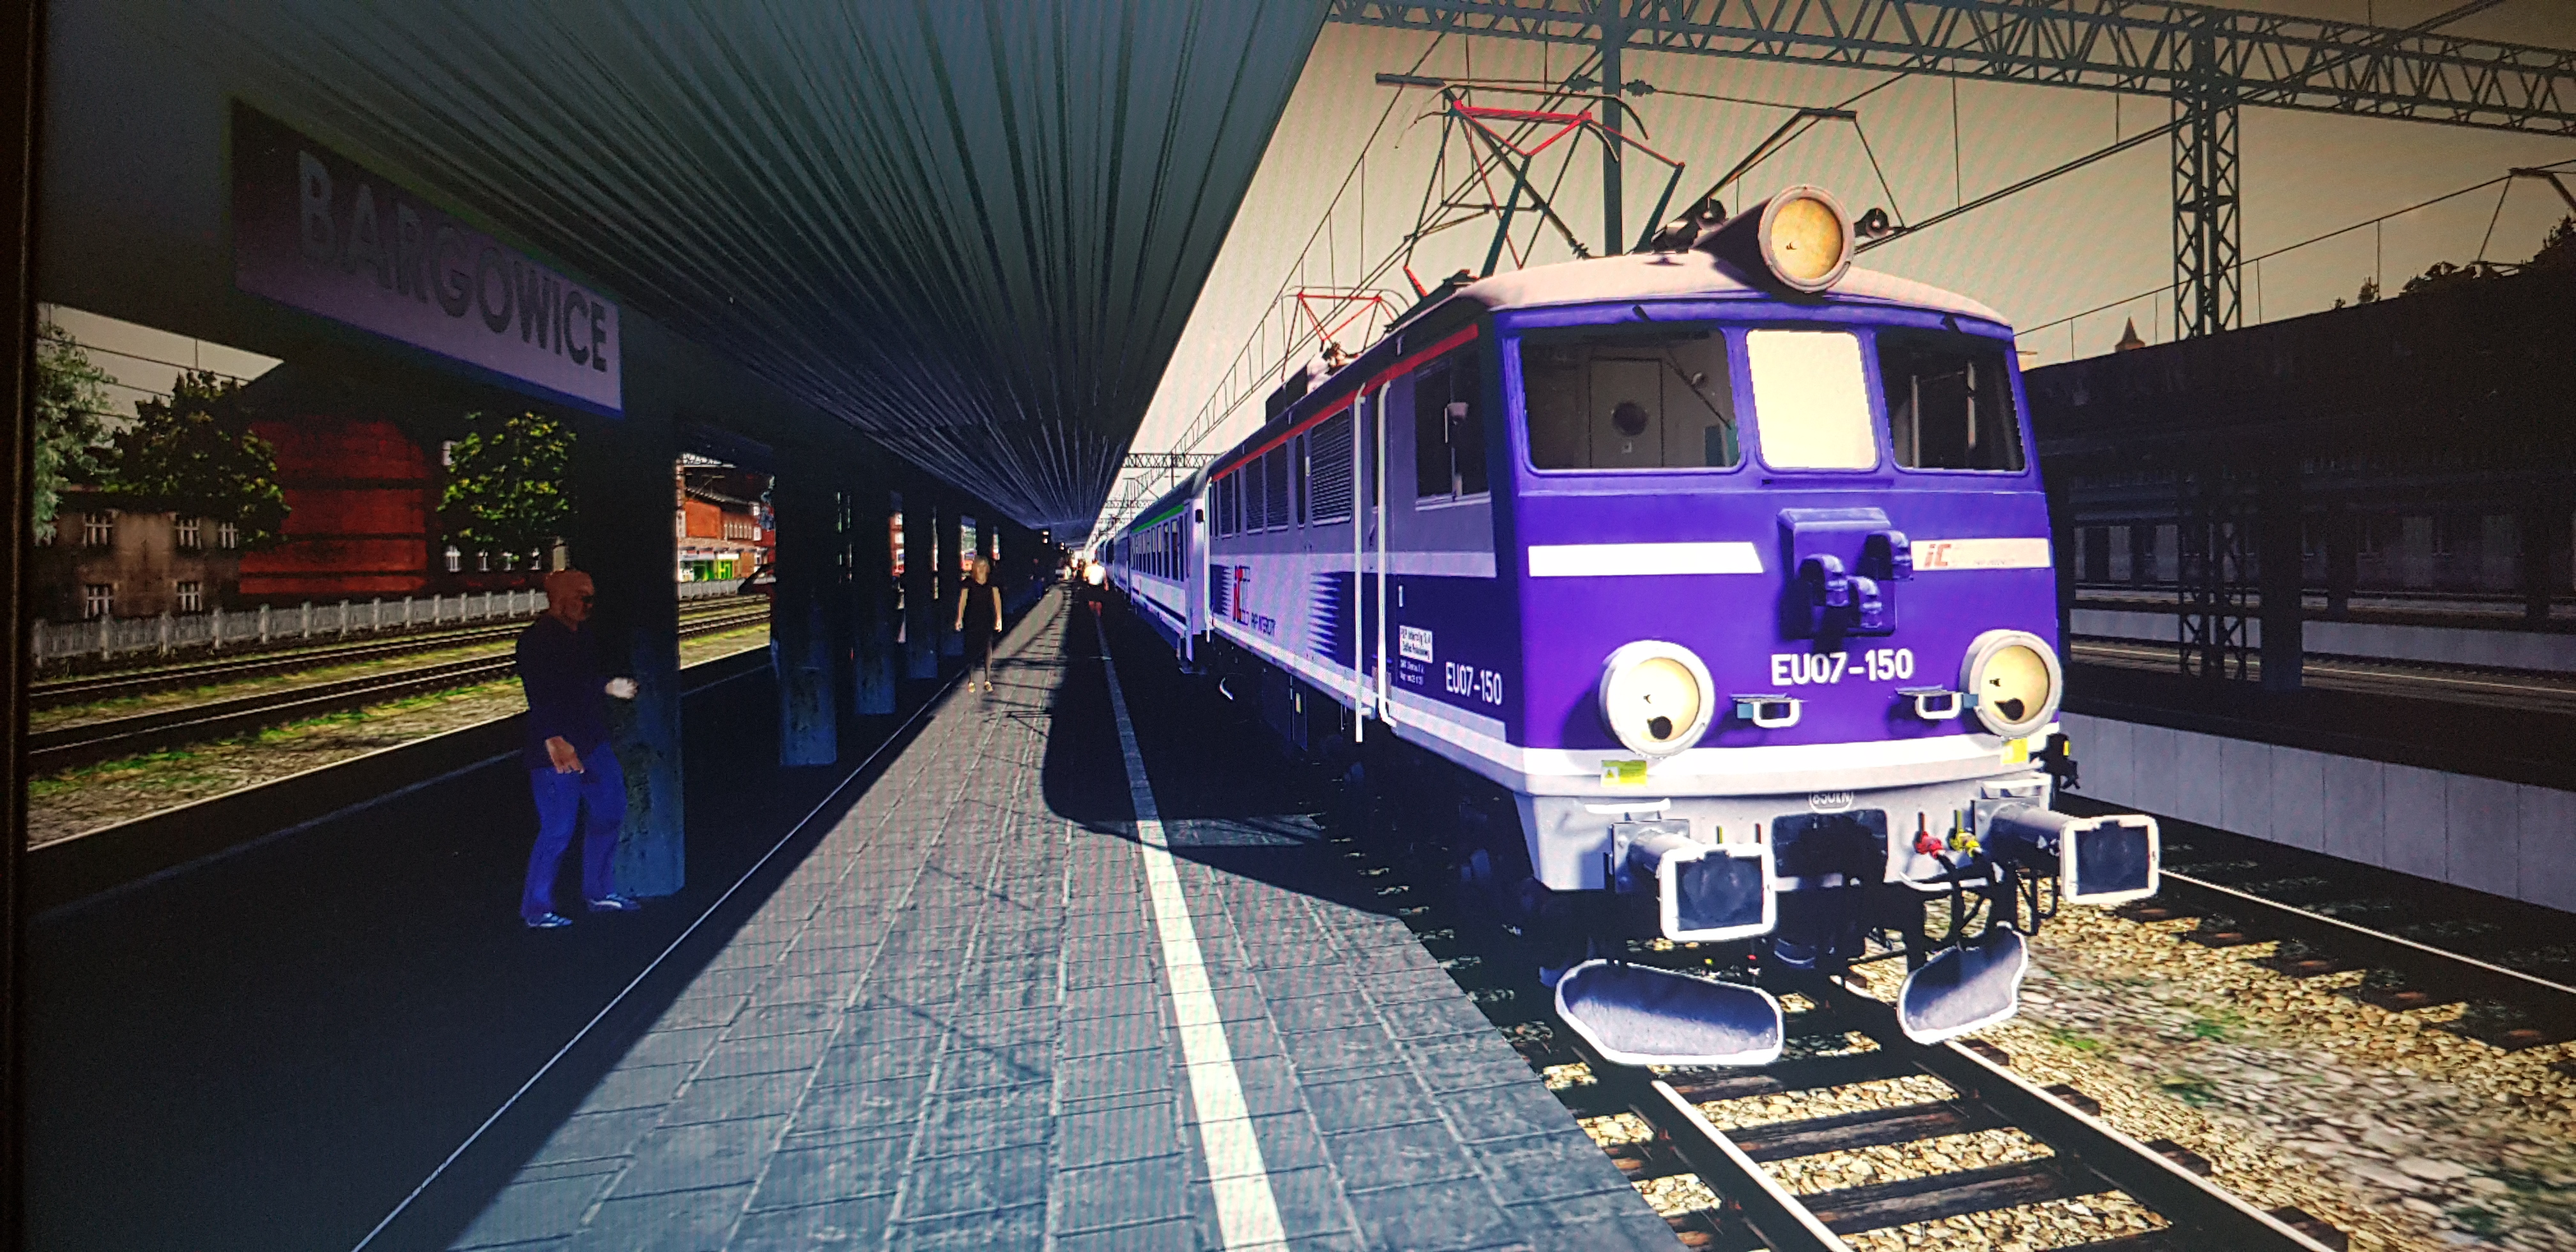
\includegraphics[width=8cm]{pictures/Dominik/20210922_232727.jpg}
  \caption{Lokomotywa EU07 - 152}
  \label{fig:3}
\end{center}
\end{figure}
\begin{figure}[!ht]
\begin{center}
 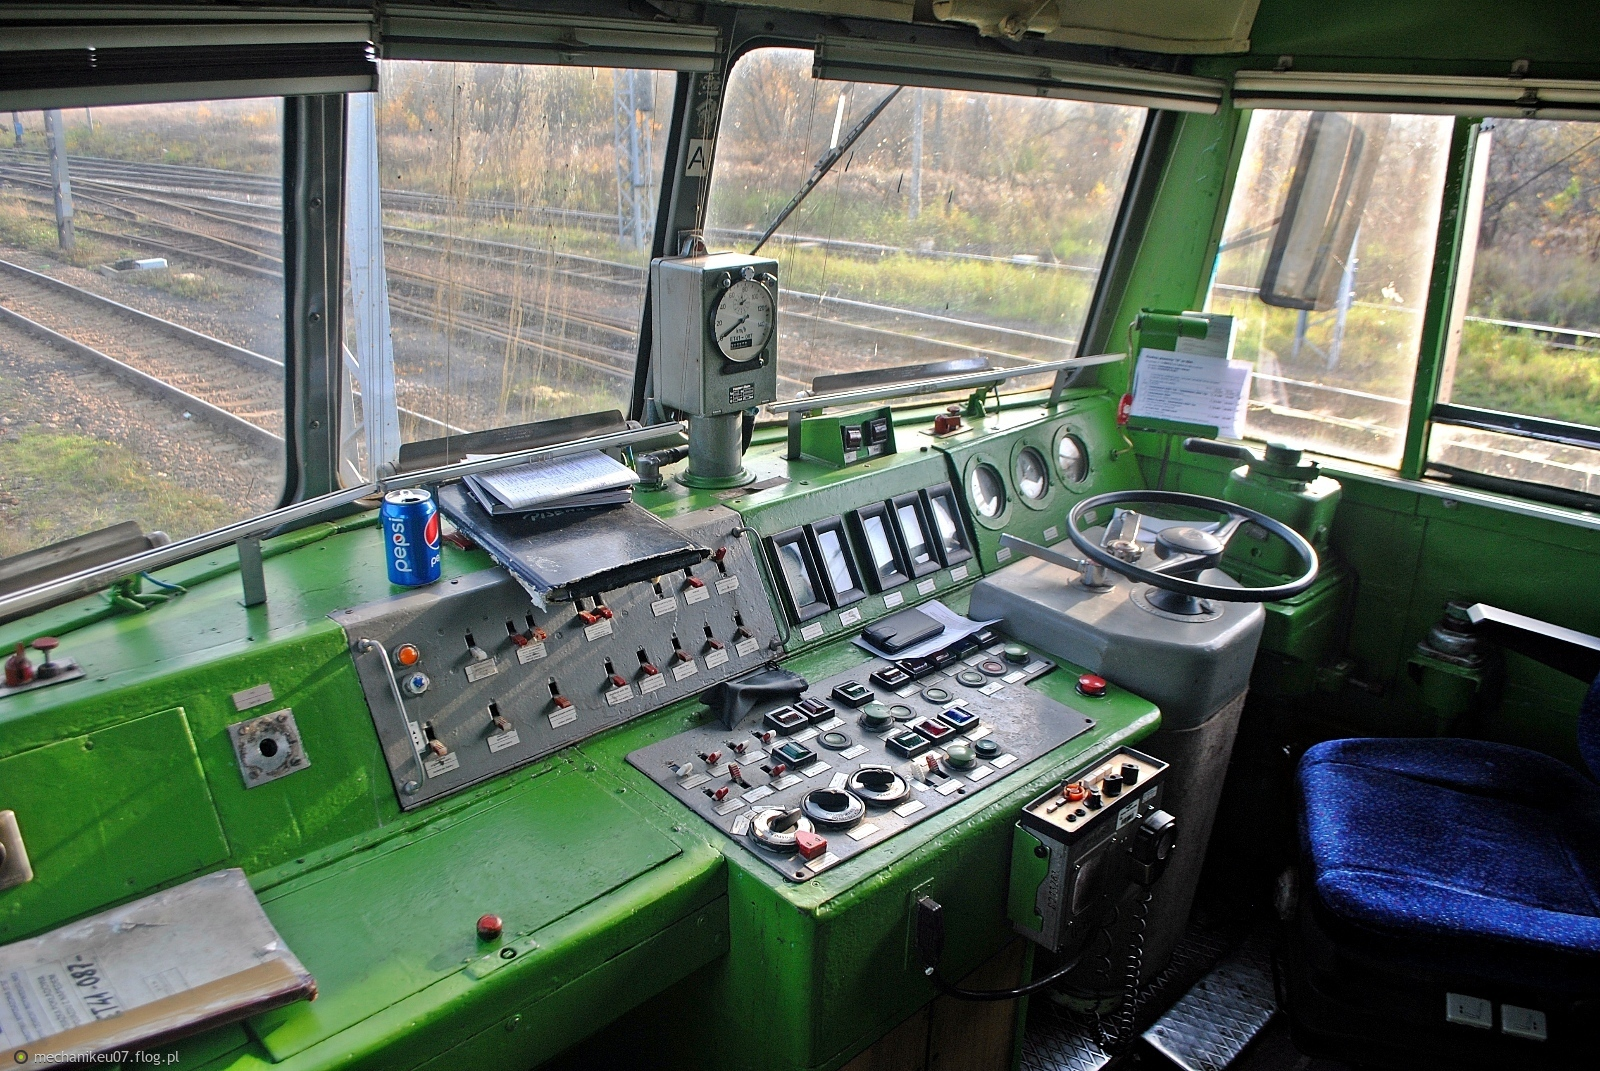
\includegraphics[width=8cm]{pictures/Dominik/9554371_kabina-et41--087.jpg}
  \caption{Wnętrze kabiny ET41 - 087}
  \label{fig:4}
\end{center}
\end{figure}
\end{center}

%%%%%%%%%%%%%%%%%%%%%%%%%%%%%%%%%%%%%%%%%%%%%%%%%%%%%%%%%%%%%%%

\subsection{Opis zdjęć:}
    \paragraph{\hspace{10mm}
    Na pierwszym zdjęciu (\ref{fig:1}) widzimy elektryczny zestaw trakcyjny (EZT) \textit{EN71-006}, o prędkości szlakowej: Vmax = 110 $\frac {km}{h}$ . Jest to prędkość, jak sama nazwa wskazuje, maksymalna dla tej konstrukcji - zawsze jest oznaczona na prędkościomierzu czerwoną kreską. Inne parametry maszyny to: m.in. dł = ok. 86 m, masa = 182 t. W żargonie kolejowym lokomotywy z serii EN są często nazwyane "Kiblem". Drugie zdjęcie (\ref{fig:2}) różni się od pierwszego tym, że jest na nim ukazany tzw. manewr, a nie pociąg - Pociąg jest na szlaku i ma ustawione reflektory tak jak na pierwszym zdjęciu. Ponadto manewr może się poruszać tylko do prędkości \underline{25$\frac {km}{h}$} i ma reflektory jak na drugim obrazku (\ref{fig:2}) obraku.}
    
    \paragraph{\hspace{10mm}A na kolejnym zdjęciu (\ref{fig:3}) widnieje lokomotywa \textit{EU07-150}, potocznie nazywana "Siódemką" (Tabela\ref{tab:Tabela}). Po obserwacji możemy zobaczyć, że ma wzniesione oba pantografy, jest to spowodowane tym ,że stoi ona na stacji. Na szlaku maszynista mechanik ma obowiązek mieć wzniesiony \underline{tylko 1 pantograf}. Zazwyczaj jest to tylni, ze względów bezpiczeństwa.}

    \paragraph{\hspace{10mm}Ostatnie zdjęcie (\ref{fig:4}) jest klasyczym przykładem wnętrza kabiny \textit{ET41 - 087}, zwyczajowa nazwa na tą lokomotywę to: "Jamnik". E oznacza, że jest to takzwany elektrowóz (patrz podrozdział 2.5). A T informuje nas, że jest to lokomotywa o przeznaczeniu towarowym, - model 41. Na  zdjęciu ulokowana jest w prawej części kabiny "Kierownica" jest po to, aby móc zwiększyć liość prądu, który płynie przez silniki - jest to zwyczajna przekładnia. \emph{Działa na zasadzie dodania gazu w samochodzie. }\textbf{Przekręcając ją w prawo musimy jednak pamiętać, aby nie dodać zbyt dużo "prądu" do silników. W przeciwnym razie zadziała system bezpieczeństwa, który spowoduje odłączenie silników z zasilania, w celu uniknięcia spalenia silników.}}

%%%%%%%%%%%%%%%%%%%%%%%%%%%%%%%%%%%%%%%%%%%%%%%%%%%%%%%%%%%%%%%

\subsection{Informacje pomocnicze o lokomotywach:}
\textbf{Klasy lokomotyw i podział:}
\begin{enumerate}
\item Ze względu na typ napędu:
    \begin{itemize}
    \item Parowe
    \item Spalinowe
    \item Elektryczne
    \end{itemize}
\item Ze względu na przeznaczenie eksploatacyjne:
    \begin{itemize}
    \item Pasażerskie
    \item Towarowe
    \item Manewrowe
    \item Uniwersalne
    \end{itemize}
\end{enumerate}

%%%%%%%%%%%%%%%%%%%%%%%%%%%%%%%%%%%%%%%%%%%%%%%%%%%%%%%%%%%%%%%

\subsection{Symbole rodzaju oraz przeznaczenia lokomotyw stosowanych obecnie w Polsce}

\begin{itemize}
\item SM – Spalinowóz Manewrowy
\item SP – Spalinowóz Pasażerski
\item SU – Spalinowóz Uniwersalny (lokomotywa przystosowana do prowadzenia pociągów towarowych i pasażerskich z możliwością ogrzewania składu)
\item ST – Spalinowóz Towarowy
\item EP – Elektrowóz Pasażerski
\item EU – Elektrowóz Uniwersalny
\item ET – Elektrowóz Towarowy
\item EM – Elektrowóz Manewrowy
\item O – parowóz Osobowy
\item P – parowóz Pośpieszny
\item T – parowóz Towarowy
\item K - (jako druga litera w oznaczeniu parowóz "kusy" (tendrzak) np. TKt48, OKl27.
\end{itemize}

%%%%%%%%%%%%%%%%%%%%%%%%%%%%%%%%%%%%%%%%%%%%%%%%%%%%%%%%%%%%%%%